% !TeX spellcheck = ru_RU
% !TEX root = vkr.tex

\section{Обзор Instrew}
\subsection{Архитектура}
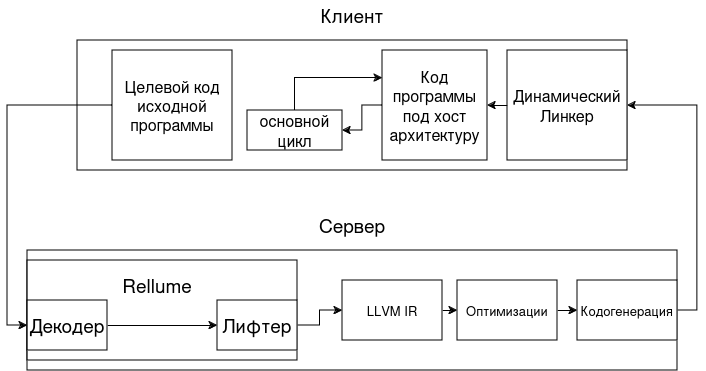
\includegraphics[width=400pt]{figures/instrew.drawio.png}
Instrew реализует клиент-сервер архитектуру:
\begin{itemize}
    \item клиент, написанный на языке C и ассемблере, и выполняющий функции:
          \begin{itemize}
              \item загрузки целевой программы в адресное пространство;
              \item эмуляции состояния процессора;
              \item отправки функций целевой программы серверу;
              \item динамической линковки ELF объектов, полученных от сервера;
              \item загрузка, разрешение символов и проведение релокаций для полученного ELF объекта;
              \item эмуляция системных вызовов;
              \item вызов функции, полученной после линковки ELF объекта;
              \item кэширование;
          \end{itemize}
    \item сервер, написанный на языке С++, выполняющий функции:
          \begin{itemize}
              \item декодирование и поднятие функции целевой программы в LLVM IR с помощью Rellume;
              \item оптимизация LLVM IR;
              \item кодогенерация;
              \item создание ELF объекта;
          \end{itemize}
\end{itemize}
% \subsection{Пример}

% \noindent Если Вам предстоит защищать учебную практику, а эти рекомендации видятся как более подходящие для защиты ВКР, то ... отмаза не засчиты\-вается, сразу учитесь делать нормально.
